  El compilador será el encargado de leer el programa de alto nivel y
traducirlo al lenguaje de bajo nivel.

  El programa resultado tendrá al principio las traducción de las
instrucciones correspondientes al bloque \texttt{do}.
  Las mismas al ser ejecutadas armarán el grafo de señales del programa.

  Al final del bloque, habrá una instrucción \texttt{halt} que cederá el
control al $dispatcher$.

  Luego estará el código correspondiente a cada función definida.
  Cada invocación a función, tendrá la referencia directa hacia la
posición en el código de la misma.

  El compilador constará de dos etapas principales.

  En la primer etapa lee el programa de alto nivel y
genera un árbol de sintaxis abstracto 
(AST)\footnote{Del inglés Abstract Syntax Tree} del mismo.
  Dicha etapa es llamada análisis sintáctico.

  Luego el ast se recorre y la segunda etapa es la generación del
código de bajo nivel.

  En la Figura \ref{fig:compiler} se puede ver la estructura más detallada
  del compilador.

\begin{figure}[hp]
\begin{center}
\caption{Diagrama del compilador}
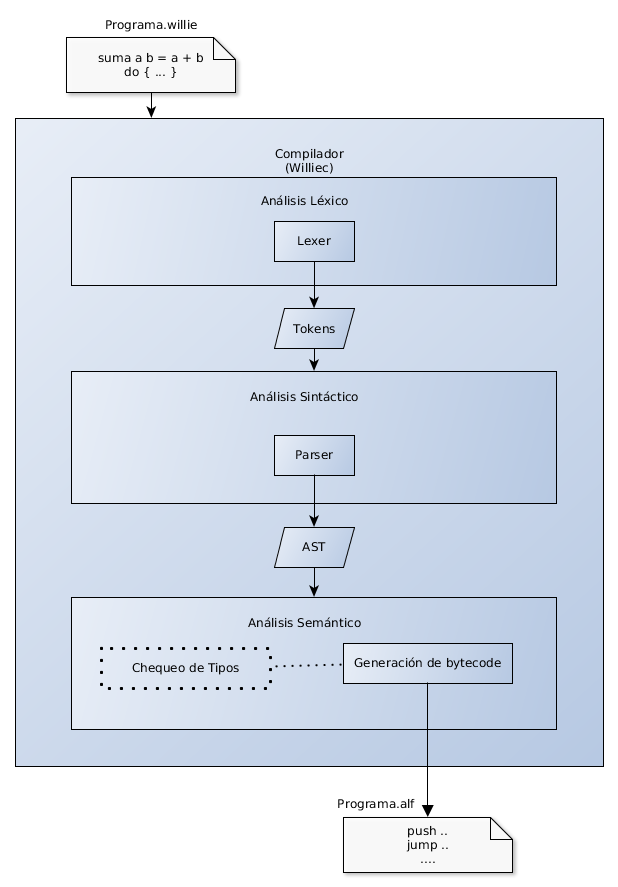
\includegraphics[width=0.9\textwidth]{graphs/compiler.png}
\label{fig:compiler}
\end{center}
\end{figure}

  TODO: Describir la Figura.

\newpage

